\chapter{Ejercicio sobre la búsqueda iterativa de óptimos}

\section{Descenso de gradiente}

El algoritmo de descenso de gradiente es una técnica general para minimizar
funciones diferenciables. Es un algoritmo iterativo basado en el cálculo del
gradiente de la función, y la actualización de cierto vector de pesos.

Formalmente, sea $w(0) \in \mathbb{R}^d$ un punto inicial, y 
$E : \mathbb{R}^d \longrightarrow \mathbb R$
una función diferenciable. Sea $\eta \in \mathbb{R}^+$. La actualización del peso en 
la $t$-ésima iteración viene definida por 

\begin{equation*}
  w(t+1) = w(t) - \eta \nabla E_{in}(w(t))
\end{equation*}

donde al parámetro $\eta$ se le conoce como tasa de aprendizaje. El algoritmo se basa
en seguir la dirección opuesta al vector gradiente pues se maximiza el decrecimiento de
la función en cada iteración. La convergencia no está garantizada en general y dependerá
de la tasa de aprendizaje escogida así como de las características de la función. 

Formalmente, esto se deduce de la expansión de Taylor de primer orden de la función:
\cite{LFD}

\begin{equation}
\begin{aligned}
\Delta E_{in} = E_{in}(w(0) + \eta \hat{v}) - E_{in}(w(0)) \\
= \eta \nabla E_{in}(w(0))^T \hat{v} + O(\eta^2) \\
= \geq - \eta \lVert \nabla E_{in}(w(0)) \rVert
\end{aligned}
\end{equation}

con $\hat{v}$ vector unitario. La igualdad se da si y sólo si

\begin{equation*}
\hat{v} = - \frac{\nabla E_{in}(w(0))}{\lVert \nabla E_{in}(w(0)) \rVert}
\end{equation*}

Una tasa de aprendizaje (demasiado) pequeña es ineficiente lejos del mínimo local. 
Por otro lado, si es demasiado grande, las oscilaciones pueden afectan a la convergencia.
Por ello, optamos por una tasa variable proporcional a la norma del gradiente.

\begin{equation*}
  \eta_t = \eta \lVert \nabla E_{in} \rVert
\end{equation*}

De esta manera, se realizan grandes pasos lejos del mínimo y pasos de menor tamaño
cerca del mínimo (donde la norma del gradiente es menor).
Además, $\eta_t$ cancela con el denominador de $\hat{v}$ definido anteriormente lo que
se sintetiza redefiniendo $\eta = \eta_t$ y hallando el opuesto del vector gradiente 
pero sin normalizar.

Como la convergencia no está garantizada en tiempo finito, necesitamos una condición de
parada como que la función a minimizar quede por debajo de cierto umbral de
error (i.e $E_{in} \leq \epsilon$) o simplemente un número máximo de iteraciones.
Combinamos ambas en la implementación ofrecida an el archivo de código:

\section{Ejercicio 1}

\textbf{Implementar el algoritmo de gradiente descendente}

Analizamos la definición de la función descrita en el código:

\begin{minted}{python}
def gradient_descent(w_ini, lr, grad_fun, fun, epsilon, max_iters, 
                     stop_cond,  hist=False):
\end{minted}

Sobre la cabecera:
\begin{itemize}
  \item \mintinline{python}{w_ini}: vector de pesos inicial
  \item \mintinline{python}{grad_fun}: gradiente de la función a minimizar
  \item \mintinline{python}{fun}: función a minimizar
  \item \mintinline{python}{epsilon}: cota de error para parar 
  \item \mintinline{python}{max_iters}: número máximo de iteraciones para parar
  \item \mintinline{python}{stop_cond(it, w, epsilon, max_iters, grad_fun, fun)}
    : función que indica cuando parar el algoritmo
    \subitem \mintinline{python}{stop_cond_maxIter}: para cuando \mintinline{python}{it <= max_iters}
    \subitem \mintinline{python}{stop_cond_error}: para cuando \mintinline{python}{fun(w[0], w[1]) \leq epsilon}
  \item \mintinline{python}{hist}: True si se desea devolver el histórico para visualización
\end{itemize}


\section{Ejercicio 2.}
Considerar la función $E(u, v) = \left( u v \cdot e^{ −u^2 −v^2 } \right) ^2$
Usar gradiente descendente para encontrar un mínimo de esta función, comenzando
desde el punto $(u, v) = (0.5, -0.5)$ y usando una tasa de aprendizaje $\eta = 0,1$.

\subsection{Cálculo análitico de \texorpdfstring{$\nabla E(u, v)$}{Lg}}

Hallamos la primera derivada parcial: 

\begin{equation}
\begin{aligned}
  \frac{\partial{E}}{\partial u}(u,v) = 2uve^{-u^2 - v^2} \cdot v \left[ e^{-u^2 - v^2} + u\cdot e^{-u^2 - v^2} \cdot 2(-u) \right] = \\
  = 2uv^2e^{2(-u^2-v^2)} - 4u^3v^2e^{2(-u^2-v^2)} = -2u (2u^2 - 1) v^2 e^{-2(u^2+v^2)}
\end{aligned}
\end{equation}

Y análogamente, $\frac{\partial{E}}{\partial u}(u,v) = -2v (2v^2 - 1) u^2 e^{-2(u^2+v^2)}$. Luego, 
\begin{equation}
  \begin{aligned}
    \nabla{E}(u,v) = \begin{pmatrix}
           \frac{\partial E}{\partial u}(u,v) \\
           \frac{\partial E}{\partial v}(u,v) 
    \end{pmatrix}  =  \begin{pmatrix}
          -2u (2u^2 - 1) v^2 e^{-2(u^2+v^2)} \\
          -2v (2v^2 - 1) u^2 e^{-2(u^2+v^2)}
    \end{pmatrix}
  \end{aligned}
\end{equation}


\subsection{Número de iteraciones con cota de error \texorpdfstring{$10^{-8}$}{Lg}}
\subsection{Coordenadas obtenidas con cota de error \texorpdfstring{$10^{-8}$}{Lg}}

Ejecutamos el algoritmo anteriormente descrito con los siguiente parámetros:

\begin{minted}{python}
eta = 0.1 
error2get = 1e-8
initial_point = np.array([0.5,-0.5])

w, it = gradient_descent(initial_point, eta, gradE, E, 
                         error2get, maxIter, stop_cond_error)
\end{minted}

La condición de parada fijada es que la función de error alcance un valor
menor o igual a $10^{-8}$, que se indica en \mintinline{python}{stop_cond_error}

\begin{itemize}
\item Numero de iteraciones: $25117$
\item Coordenadas obtenidas: $(0.0100, -0.0100)$
\end{itemize}


En la siguiente figura visualizamos el desplazamiento hacia el mínimo: 

\begin{figure}[H]
\centering
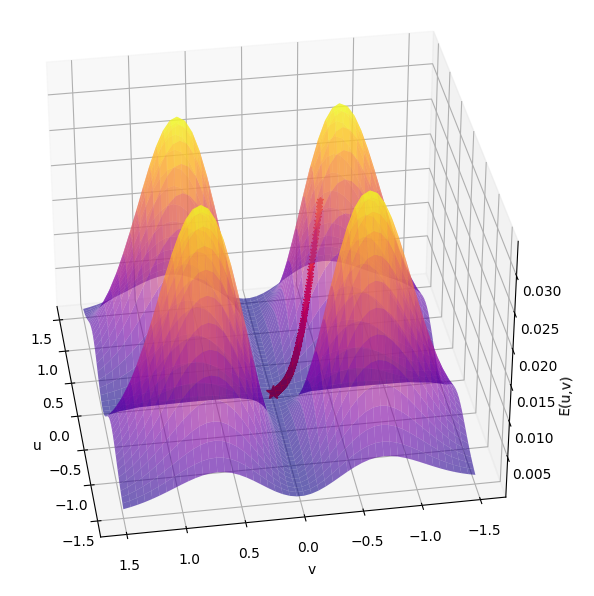
\includegraphics[width=0.5\textwidth]{Figure_1.png}
\caption{Descenso de gradiente sobre E}
\end{figure}

\section{Ejercicio 3}

Consideramos la función  $f(x,y) = x^2 + 2y^2 + 2 \sin (2 \pi x) \sin (\pi y)$.
\textbf{Aplicar gradiente descendente para minimizar $f$}

\subsection{Dependencia de la tasa de aprendizaje}

Usar como punto inicial $(x_0 = -1, y_0 = 1)$, tasa de aprendizaje $\eta = 0,01$
y un máximo de $50$ iteraciones. Generar un gráfico de cómo desciende el valor
de la función con las iteraciones. Repetir el experimento pero usando 
$\eta =0,1$, comentar las diferencias y su dependencia de $\eta$.  

En primer lugar, calculamos analíticamente el gradiente de $f$.

\begin{equation}
\begin{aligned}
  \nabla f(x,y) = \begin{pmatrix}
  \frac{\partial }{\partial x} f(x,y) \\
  \frac{\partial }{\partial y} f(x,y)
  \end{pmatrix} = \begin{pmatrix}
   2x + 4\pi sen(\pi y)cos(2\pi x) \\
   4y + 2\pi sen(\pi x)cos(\pi y)
  \end{pmatrix}
\end{aligned}
\end{equation}

En este caso la condición de parada es el máximo de iteraciones, por lo que
que ejecutamos el algoritmo con la función de condición de parada
\mintinline{python}{stop_cond_maxIter}

\begin{minted}{python}
eta = 0.01 
maxIter = 50
initial_point = np.array([-1, 1])

ws, it = gradient_descent(initial_point, eta, gradf, f, None, maxIter,
                         stop_cond_maxIter, hist=True)

\end{minted}

Así, para $\eta=0.01$ y un máximo de $50$ iteraciones, las coordinadas finales
son $(-1.2178, 0.4134)$ donde $f$ toma el valor $-0.0623$

\begin{figure}[H]
\centering
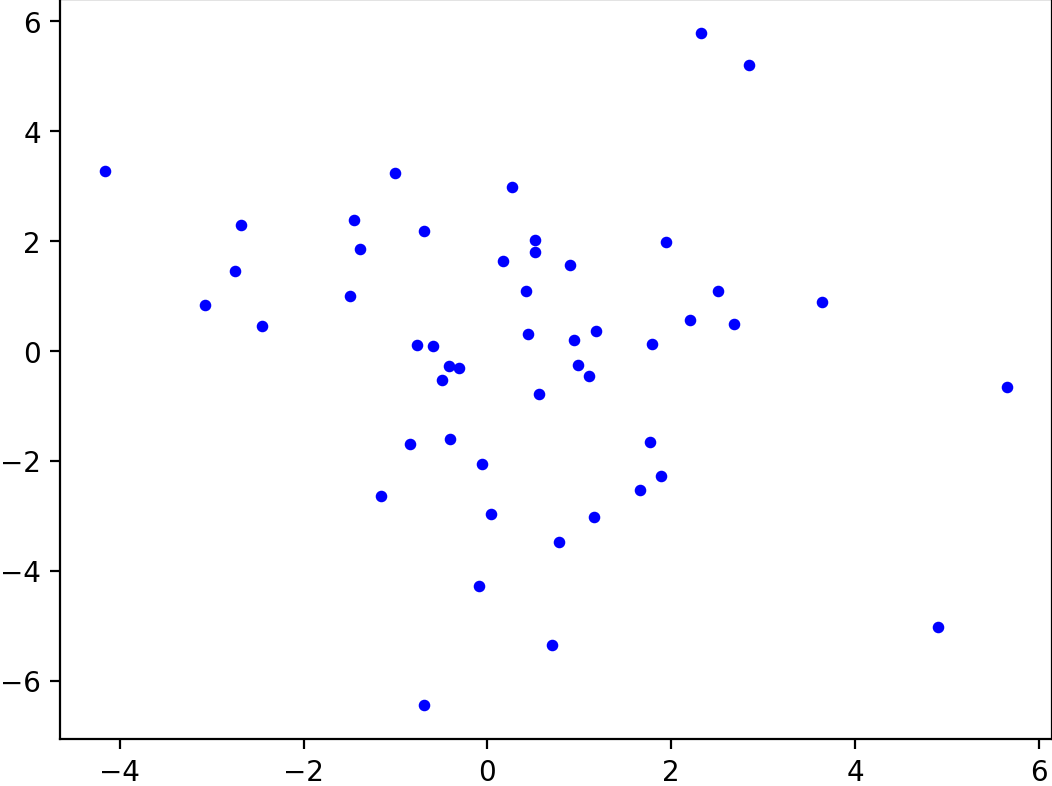
\includegraphics[width=0.6\textwidth]{Figure_2.png}
\caption{Descenso del gradiente sobre f con $\eta=0.01$}
\end{figure}

De igual manera para $\eta=0.1$ las coordenadas finales obtenidas son 
$(-0.1155, 0.1610)$ y visualizamos el descenso en la siguiente figura:

\begin{figure}[H]
\centering
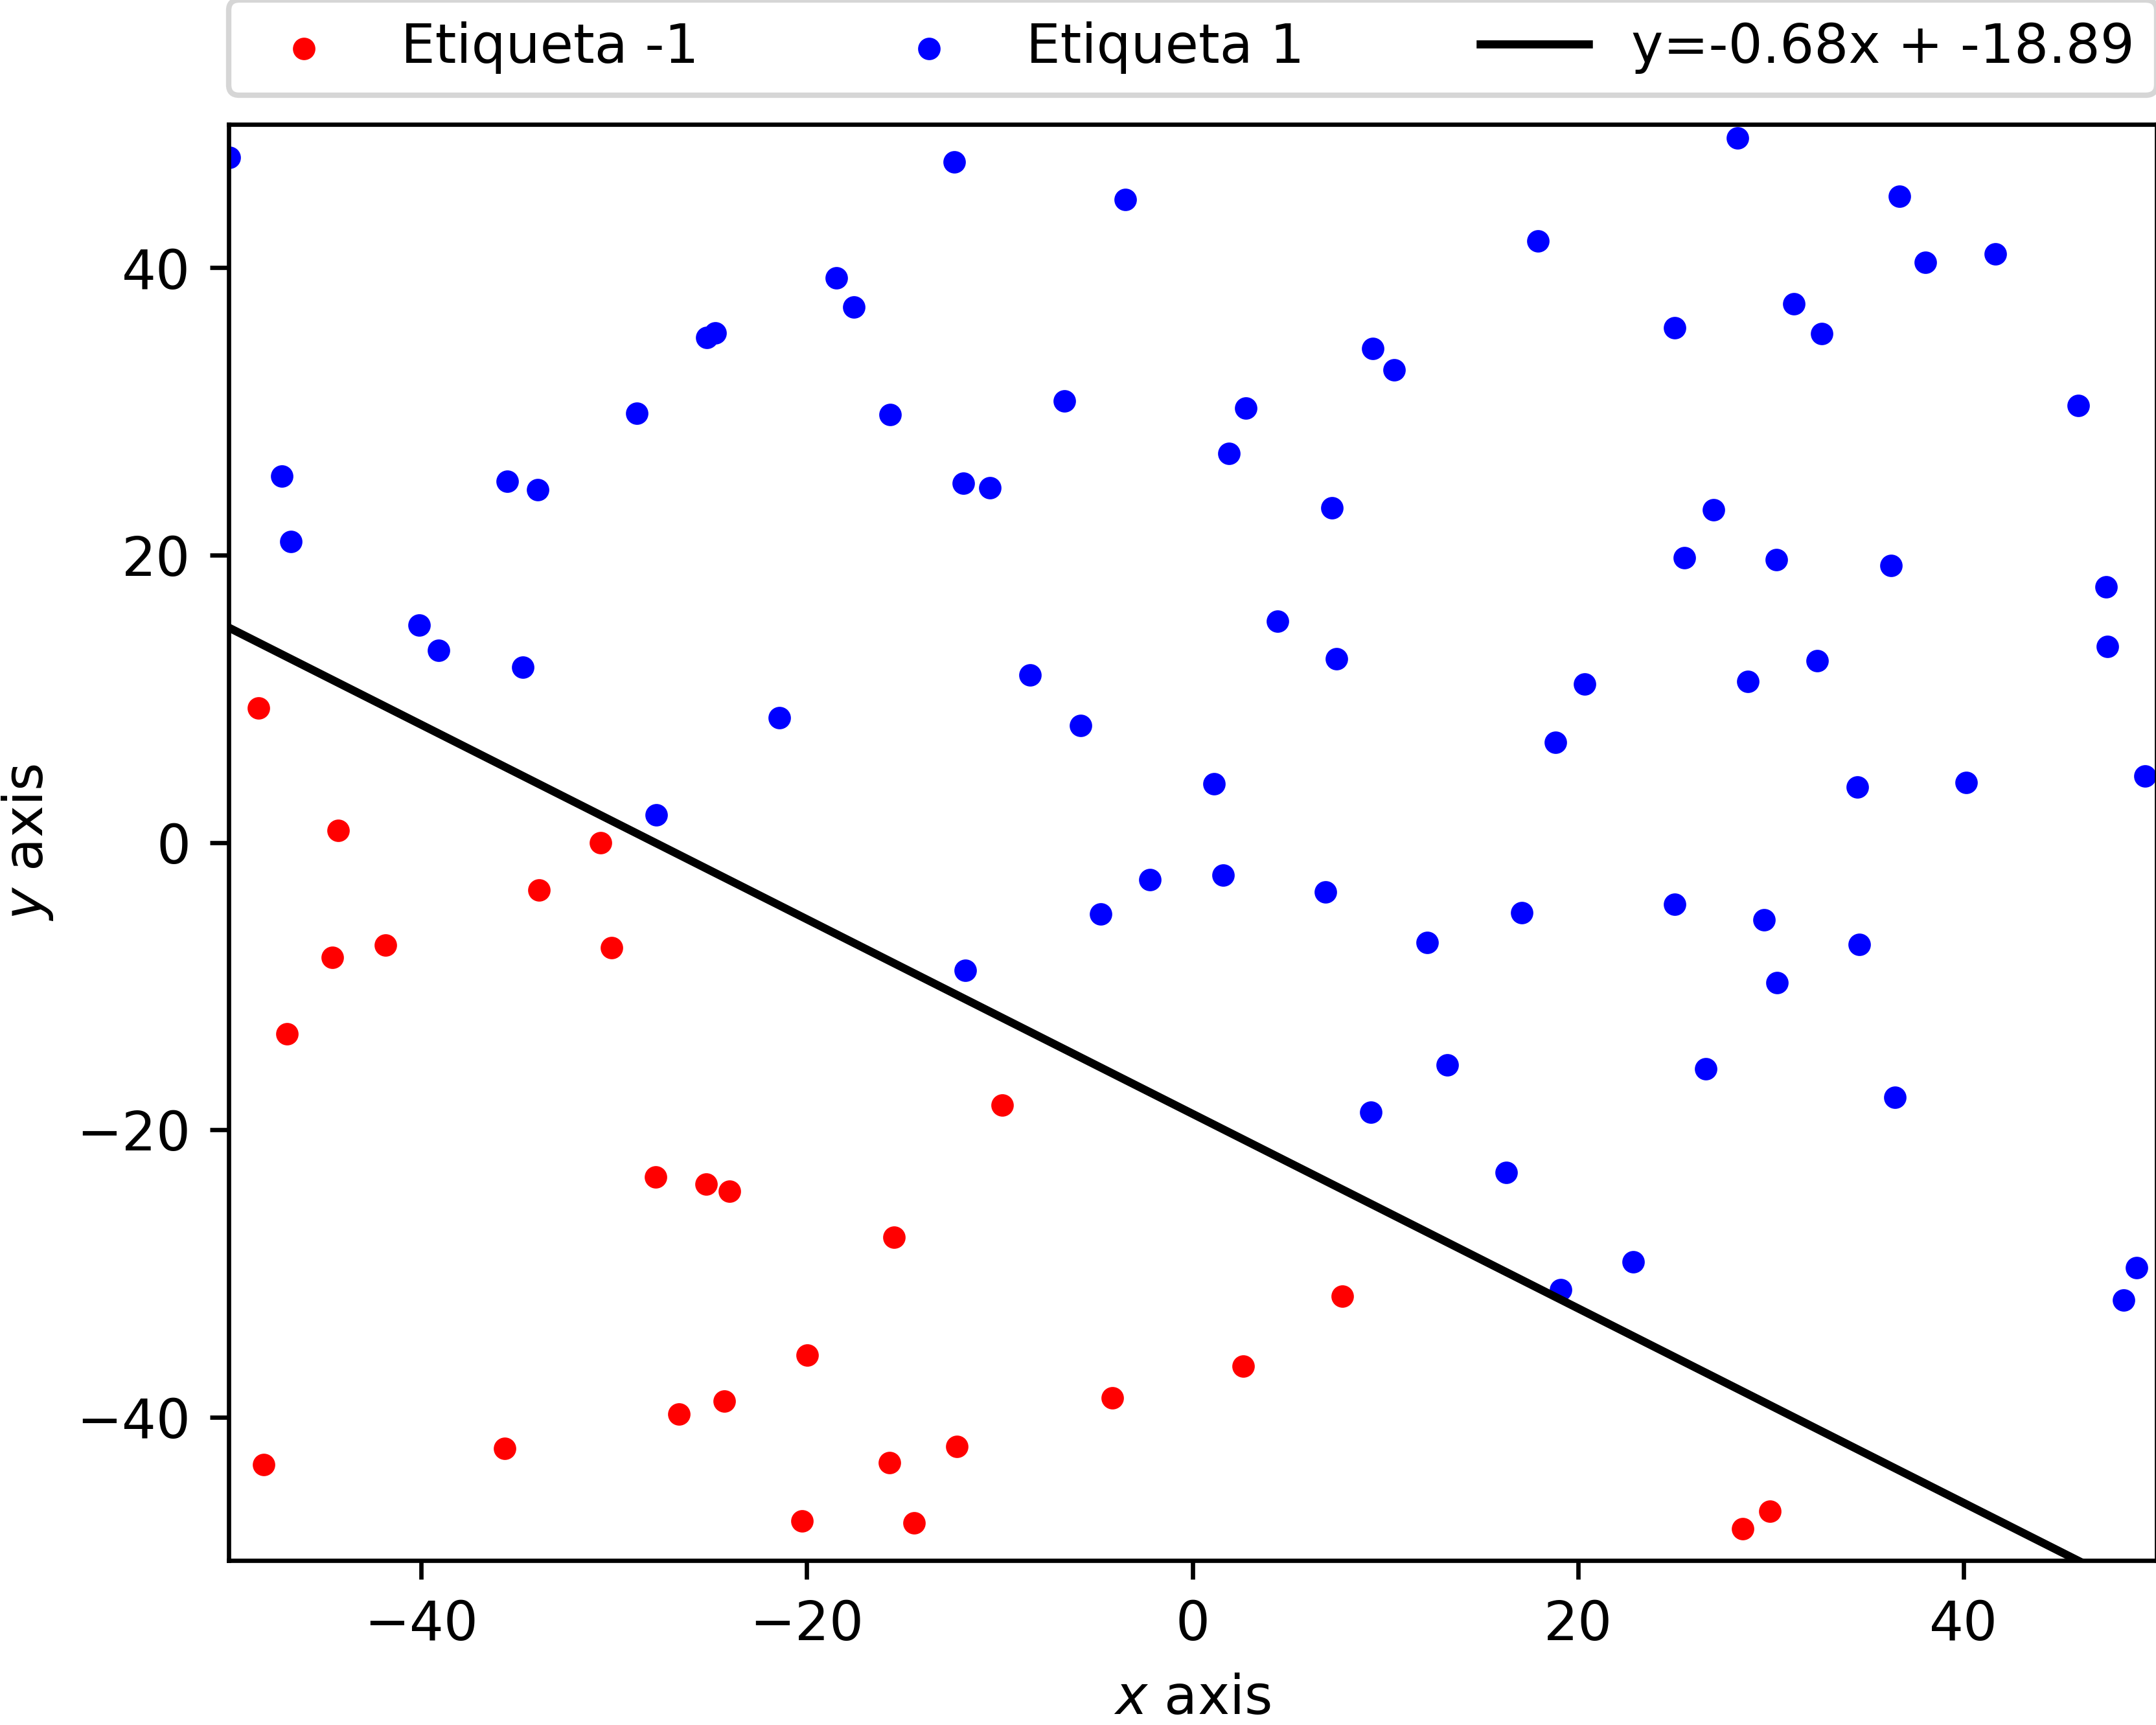
\includegraphics[scale=0.75]{Figure_3.png}
\caption{Descenso del gradiente sobre f con $\eta=0.1$}
\end{figure}

Como se observa en la figura, la tasa de aprendizaje es demasiado alta,
provocando oscilaciones que saltan el mínimo. De hecho, una inspección del
vector de puntos \mintinline{python}{ws} revela que en la $43$-ésima iteración
alcanza el mínimo valor de las $50$ iteraciones, pero que luego sigue oscilando y
termina en la última iteración con un valor mayor.

La comparación entre las oscilaciones con $\eta=0.1$ y el descenso adecuado con 
$\eta=0.01$ quedan reflejadas en la siguiente figura.

\begin{figure}[H]
  \centering
  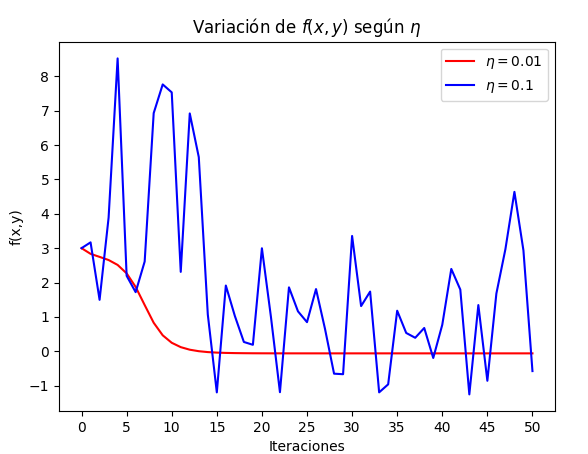
\includegraphics[width=0.6\textwidth]{Figure_4.png}
  \caption{Comparación de $f(x,y)$ para $\eta=0.01$ y $\eta=0.1$}
\end{figure}

% Análogamente, si elegimos un valor menor, i.e $\eta = 0.05$, obtendremos
% un descenso más lento (más ineficiente) para el mismo número de iteraciones ($50$)
% en comparación con $\eta = 0.01$, como podemos observar en la siguiente gráfica:

% \begin{figure}[H]
%   \centering
%  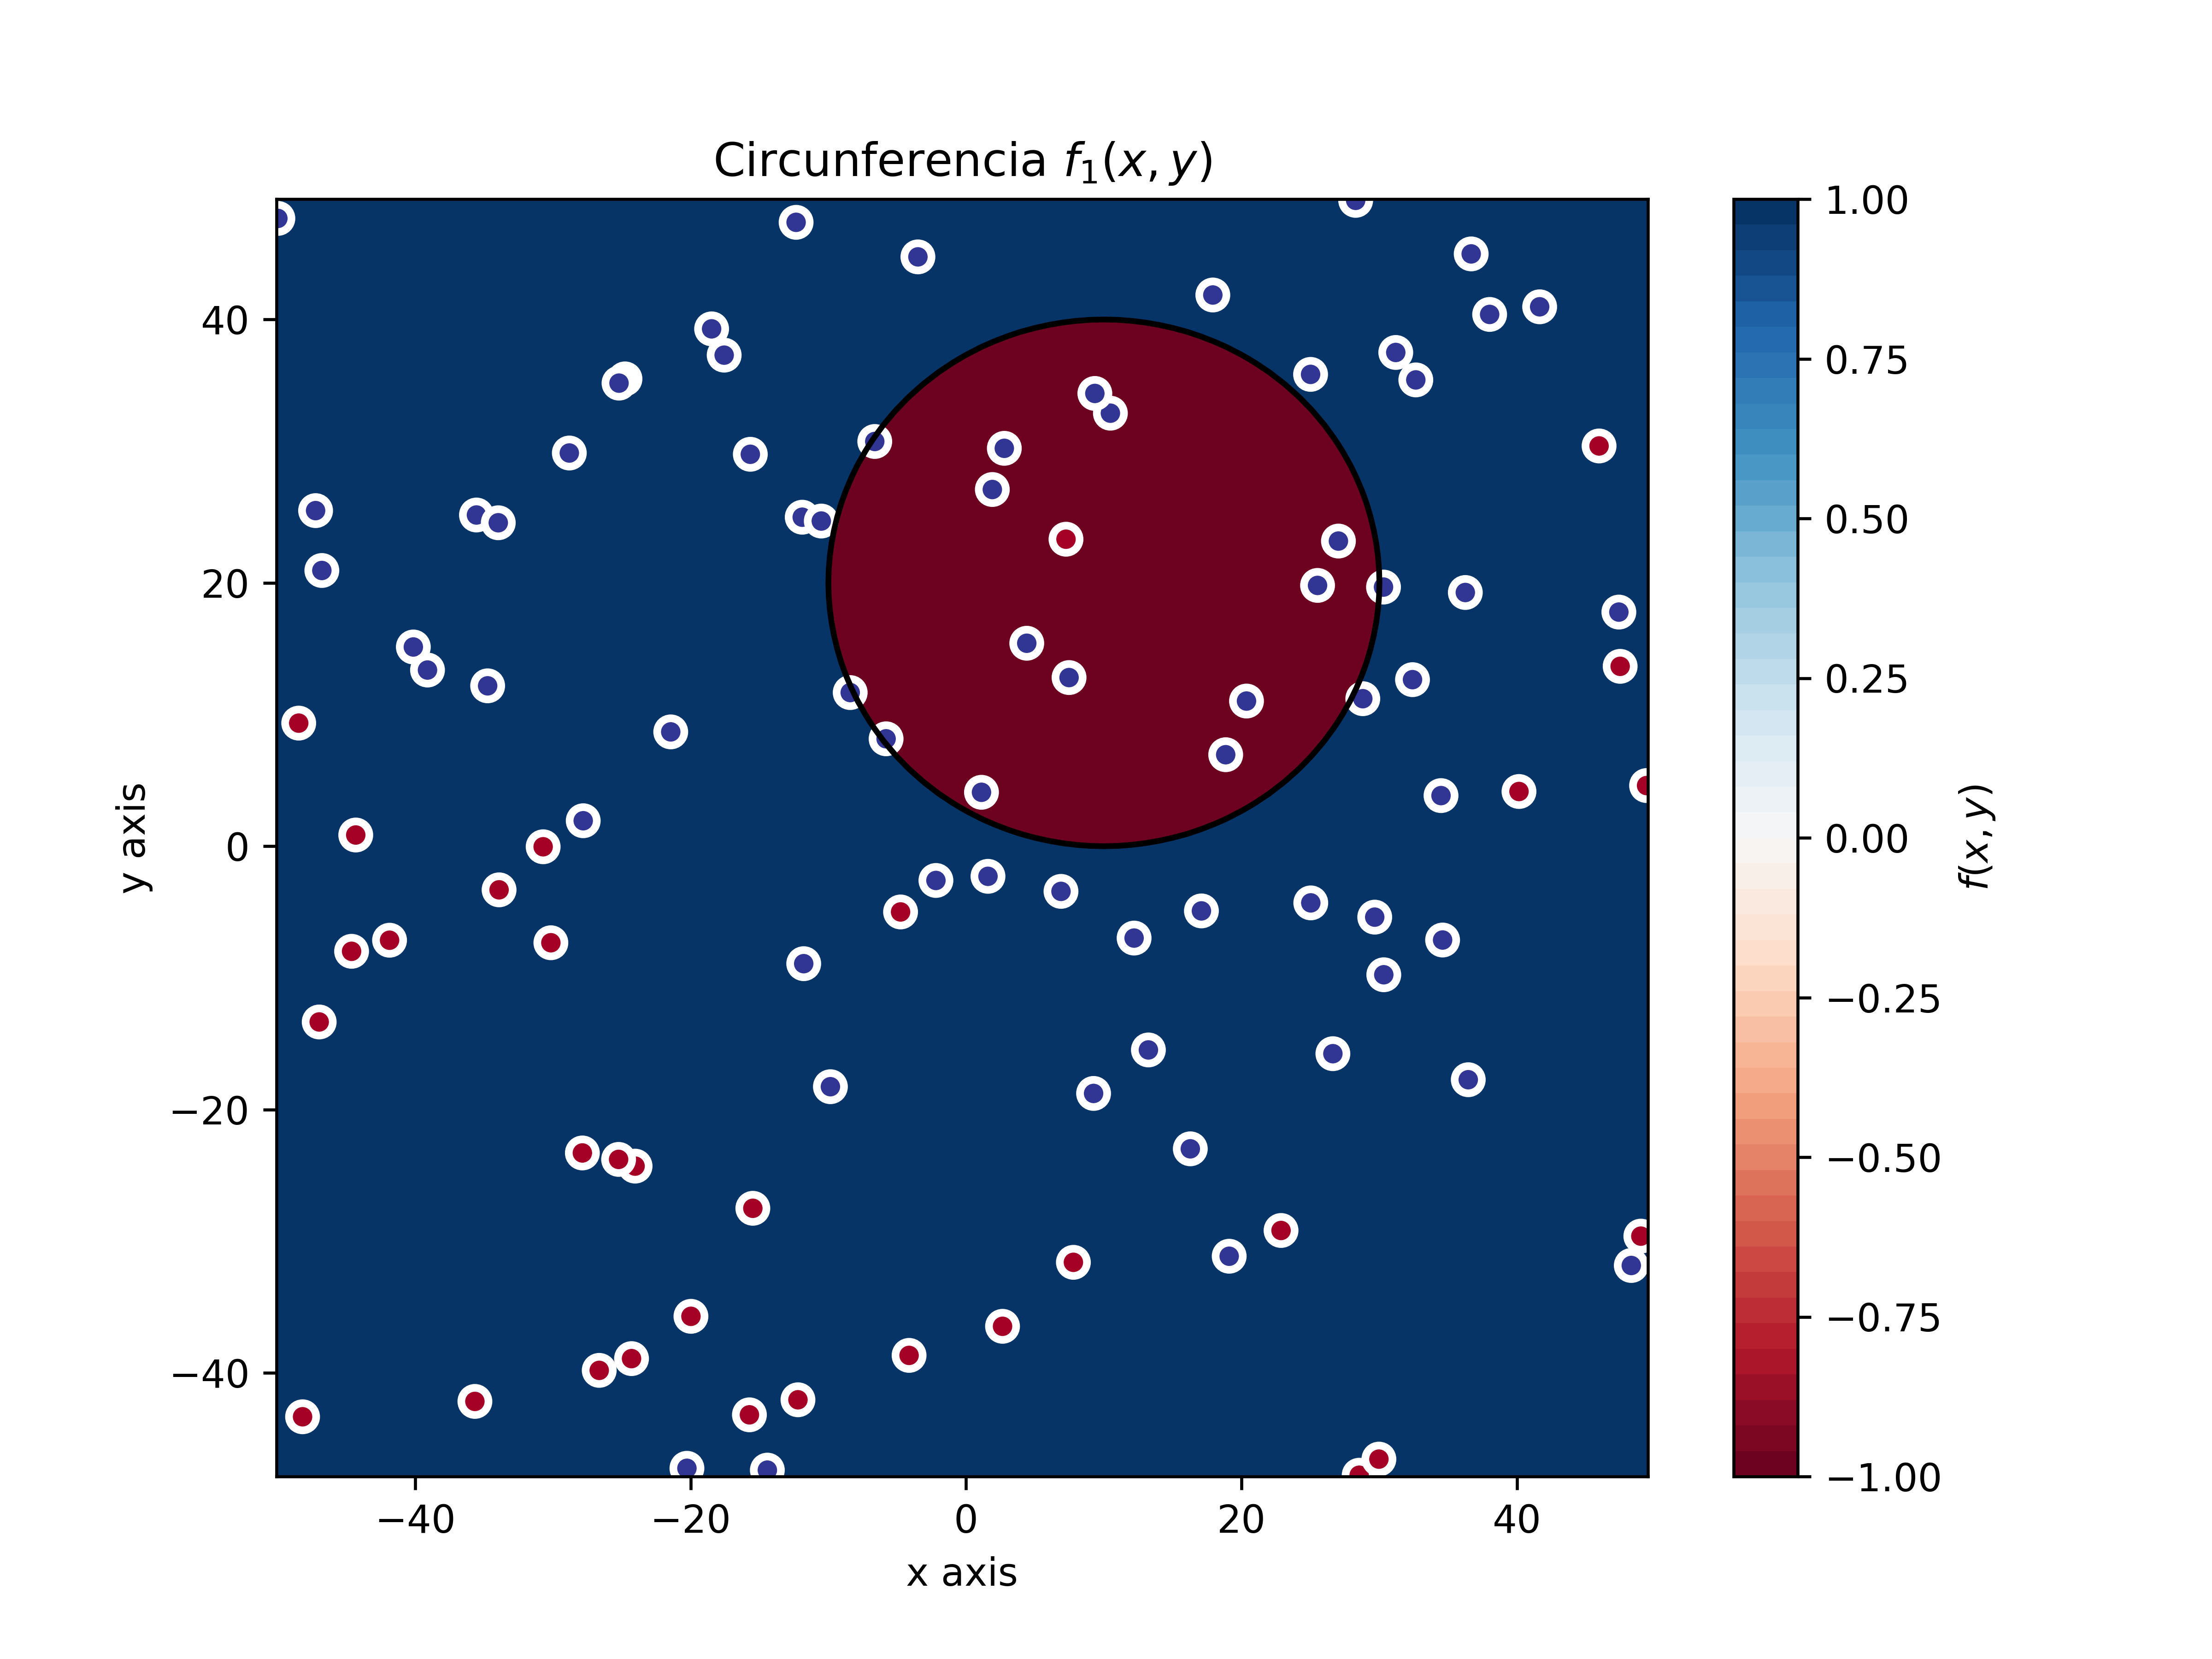
\includegraphics[scale=0.6]{Figure_5.png}
%  \caption{Comparación de $f(x,y)$ para $\eta=0.01$ y $\eta=0.05$}
% \end{figure}


\subsection{Tabla de mínimos según punto inicial y tasa de aprendizaje}

Obtener el valor mínimo y los valores de las variables $(x, y)$ en donde se
alcanzan cuando el punto de inicio se fija en: $(-0.5, -0.5)$, $(1, 1)$, $(2.1,-2.1)$,
$(-3, 3)$, $(-2, 2)$.
Generar una tabla con los valores obtenidos, empleando el máximo número de
iteraciones ($50$) y las tasas de aprendizaje del anterior apartado ($\eta=0.01$ y 
$\eta = 0.1$). Comentar la dependencia del punto inicial.

\begin{table}[!ht]
    \caption {Valor mínimo para $\eta = 0.1$} \label{tab:title} 
    \centering
    \begin{tabular}{lll}
    \toprule
        Punto inicial & Coordenadas mínimo & Valor mínimo f(x,y) \\ \midrule
        (-0.5, -0.5) & (0.2848,-0.5553) & -1.2250 \\
        (1, 1) & (0.3018,-0.4257) & -1.3902 \\ 
        (2.1, -2.1) & (-0.2320,0.2831) & -1.3293 \\
        (-3, 3) & (0.1816,-0.3152) & -1.2883 \\
        (-2, 2) & (0.2428,-0.3121) & -1.4061 \\ \bottomrule
    \end{tabular}
\end{table}

\begin{table}[!ht]
    \caption {Valor mínimo para $\eta = 0.01$} \label{tab:title2} 
    \centering
    \begin{tabular}{lll}
    \toprule
        Punto inicial & Coordenadas mínimo & Valor mínimo f(x,y) \\ \midrule
        (-0.5, -0.5) & (-0.7308,-0.4144) & -1.0366 \\ 
        (1, 1) & (0.7308,0.4144) & -1.0366 \\ 
        (2.1, -2.1) & (1.6651,-1.1728) & 4.6338 \\ 
        (-3, 3) & (-2.1888,0.5868) & 3.6942 \\ 
        (-2, 2) & (-1.6643,1.1713) & 4.6337 \\ \bottomrule
    \end{tabular}
\end{table}

Es claro a partir de estos datos que el algoritmo de gradiente Descendente tiende
hacia un mínimo local que dependerá del punto inicial. En general, en este caso,
la tasa de aprendizaje mayor $\eta=0.1$ proporciona un valor mínimo más regular
(en torno a $-1.25$) que la tasa $\eta=0.01$. 

\section{Ejercicio 4}

\textbf{¿Cuál sería su conclusión sobre la verdadera dificultad de encontrar el mínimo
global de una función arbitraria?}

A partir del experimento anterior, confirmamos empíricamente que el mínimo local
que encuentra el algoritmo de gradiente Descendente depende fuertemente tanto
del punto inicial como de la tasa de aprendizaje. No podemos garantizar que este
mínimo sea global a no ser que la función sea convexa. Esto último sucede en los casos
de la función de error cuadrático medio de la regresión lineal así como en el 
error de entropía cruzada de la regresión logística. 
Esto significa que al minimizar estas medidas de error convexas con este
algoritmo, no se estancará en un mínimo local.